%____________________________________________________________________________||
\section{Interpretation in Dark Matter models} \label{sec:darkmatter}



\subsection{Light flavour models} \label{sec:dm_lightjet}

The light flavour simplified models consist of a DM particle \pchi of mass
\mchi that is a Diract fermion, and a spin-1 (vector or axial-vector) or spin-0
(scalar or pseudoscalar) mediating particle \pphi of mass \mphi in an
$s$-channel. The couplings of the mediator with the standard model and dark
matter particles are given by \gsm and \gdm, respectively. The recommendations
by the DM Forum on the choice of couplings is \gsm$=1$,\gdm$=1$ for
(pseudo)scalar models, and \gsm$=0.25$,\gdm$=1$ for (axial-)vector models.
Assuming that no additional visible or invisible particles contribute to the decay 
of the mediator, we impose the minimal width determined by the choice of couplings. 
An example Feynman diagram is shown in Fig.~\ref{fig:DMfeynman}.



Assuming 2~\ifb of data we list the cross sections, yields and selection 
efficiencies for the four light jet models in
Tables~\ref{tab:dm_V_g1_2fb}-\ref{tab:dm_P_g1_2fb}. The signal selection
efficiencies are around $\sim 1$\% for mass points near the expected exclusion
region, and are correspondingly larger (smaller) for higher (lower) mass points.
The asymmetric and monojet categories are seen to almost double the acceptance
to these models compared to the Run~1 symmetric categories alone, justifying the
inclusion of these selections into the analysis.




\clearpage 
\begin{table}
\small
\centering
\begin{tabular}{lllllll}
\hline
$m_\phi$ & $m_\chi$ & $\sigma$ [pb] & Yield (sym) & Yield (asy) & Yield (mon) & Efficiency [\%] \\ \hline
10000     &   100       &   1.99e-04  &   0.00      &   0.00      &   0.00      &   1.45      \\ 
10000     &   150       &   1.80e-04  &   0.00      &   0.00      &   0.00      &   1.59      \\ 
10000     &   500       &   7.68e-05  &   0.00      &   0.00      &   0.00      &   2.11      \\ 
10000     &   50        &   2.09e-04  &   0.00      &   0.00      &   0.00      &   1.12      \\ 
1000      &   1000      &   5.04e-03  &   0.06      &   0.07      &   0.13      &   2.38      \\ 
1000      &   100       &   2.73e+01  &   179.52    &   190.01    &   383.56    &   1.31      \\ 
1000      &   150       &   2.62e+01  &   160.27    &   208.11    &   403.66    &   1.40      \\ 
1000      &   1         &   2.71e+01  &   160.57    &   203.17    &   434.80    &   1.40      \\ 
1000      &   500       &   4.97e+00  &   33.21     &   47.36     &   81.68     &   1.55      \\ 
100       &   10        &   5.93e+04  &   7589.50   &   19108.63  &   31108.83  &   0.05      \\ 
100       &   1         &   5.91e+04  &   14800.01  &   12847.15  &   11821.32  &   0.03      \\ 
100       &   50        &   3.88e+03  &   539.13    &   1807.91   &   4031.74   &   0.08      \\ 
10        &   100       &   5.54e+01  &   103.87    &   126.63    &   248.14    &   0.41      \\ 
10        &   10        &   5.17e+04  &   1145.90   &   332.97    &   2451.58   &   0.00      \\ 
10        &   150       &   1.37e+01  &   47.10     &   58.73     &   111.65    &   0.76      \\ 
10        &   500       &   1.41e-01  &   1.16      &   1.34      &   2.76      &   1.78      \\ 
10        &   50        &   4.67e+02  &   230.50    &   378.34    &   743.68    &   0.14      \\ 
2000      &   1         &   1.21e+00  &   11.66     &   12.00     &   24.85     &   1.92      \\ 
200       &   10        &   6.95e+03  &   5415.53   &   7354.07   &   15915.05  &   0.20      \\ 
200       &   150       &   2.67e+01  &   73.94     &   84.18     &   215.47    &   0.67      \\ 
200       &   1         &   7.31e+03  &   5121.26   &   7686.21   &   18636.29  &   0.20      \\ 
200       &   1         &   7.31e+03  &   6238.76   &   9708.29   &   17140.23  &   0.22      \\ 
200       &   50        &   7.21e+03  &   4068.85   &   7543.76   &   16796.86  &   0.19      \\ 
20        &   1         &   3.89e+06  &   72829.16  &   0.00      &   0.00      &   0.00      \\ 
300       &   100       &   1.92e+03  &   3361.32   &   3813.36   &   9551.46   &   0.42      \\ 
300       &   10        &   2.14e+03  &   3897.55   &   4065.27   &   11657.41  &   0.44      \\ 
300       &   150       &   2.65e+02  &   500.37    &   656.11    &   1441.81   &   0.47      \\ 
300       &   1         &   2.07e+03  &   3791.08   &   4448.85   &   9664.55   &   0.41      \\ 
300       &   50        &   2.04e+03  &   3769.22   &   4258.83   &   10451.88  &   0.43      \\ 
500       &   100       &   3.42e+02  &   966.21    &   1385.64   &   3075.59   &   0.76      \\ 
500       &   10        &   3.45e+02  &   1118.46   &   1620.52   &   2888.59   &   0.78      \\ 
500       &   150       &   3.28e+02  &   985.14    &   1458.16   &   2740.83   &   0.75      \\ 
500       &   1         &   3.23e+02  &   1325.55   &   1776.04   &   3250.20   &   0.94      \\ 
500       &   500       &   1.97e-01  &   1.54      &   1.88      &   3.85      &   1.76      \\ 
500       &   50        &   3.43e+02  &   1013.67   &   1413.07   &   3283.48   &   0.79      \\ 
50        &   10        &   3.83e+05  &   4924.12   &   9435.89   &   10145.19  &   0.00      \\ 
50        &   1         &   3.96e+05  &   16034.59  &   32044.78  &   15910.13  &   0.01      \\ 
50        &   50        &   6.32e+02  &   360.15    &   560.45    &   947.73    &   0.14      \\ 
\hline
\end{tabular}
\caption{Cross section, yields at 2~\ifb (split according to symmetric, asymmetric, and monojet categories), and total selection efficiency for the vector \DMj samples wtih $g_{\rm DM}=$0.25.}
\label{summaryTableAN_DMV_xs10_g0p25_2p1fb_exp}
\end{table}
 \clearpage
\begin{table}
\small
\centering
\begin{tabular}{lllllll}
\hline
$m_\phi$ & $m_\chi$ & $\sigma$ [pb] & Yield (sym) & Yield (asy) & Yield (mon) & Efficiency [\%] \\ \hline
10000     &   100       &   1.62e-04  &   0.00      &   0.00      &   0.00      &   1.56      \\ 
10000     &   150       &   1.38e-04  &   0.00      &   0.00      &   0.00      &   1.72      \\ 
10000     &   1         &   2.43e-04  &   0.00      &   0.00      &   0.00      &   1.12      \\ 
1000      &   150       &   2.42e+01  &   141.00    &   188.79    &   381.67    &   1.40      \\ 
1000      &   500       &   3.77e-01  &   2.79      &   3.55      &   7.73      &   1.78      \\ 
1000      &   50        &   2.63e+01  &   157.95    &   181.07    &   406.42    &   1.35      \\ 
100       &   100       &   2.55e+01  &   56.95     &   79.57     &   146.42    &   0.53      \\ 
100       &   10        &   5.66e+04  &   9938.63   &   22146.95  &   32316.52  &   0.05      \\ 
100       &   1         &   5.91e+04  &   17332.64  &   5289.88   &   18352.75  &   0.03      \\ 
10        &   100       &   2.05e+01  &   38.47     &   53.97     &   114.44    &   0.48      \\ 
10        &   10        &   2.05e+04  &   53.71     &   1787.34   &   1963.65   &   0.01      \\ 
10        &   500       &   4.17e-02  &   0.38      &   0.42      &   0.83      &   1.87      \\ 
10        &   50        &   1.88e+02  &   186.18    &   151.23    &   444.36    &   0.20      \\ 
2000      &   1         &   1.23e+00  &   12.53     &   13.56     &   24.58     &   1.97      \\ 
2000      &   50        &   1.18e+00  &   10.80     &   12.34     &   27.25     &   2.03      \\ 
200       &   10        &   7.21e+03  &   4959.50   &   8237.15   &   18440.27  &   0.21      \\ 
200       &   150       &   8.03e+00  &   22.90     &   32.03     &   67.88     &   0.73      \\ 
200       &   1         &   7.47e+03  &   6195.99   &   8950.18   &   15562.51  &   0.20      \\ 
20        &   10        &   2.93e+04  &   333.66    &   1032.22   &   709.73    &   0.00      \\ 
300       &   150       &   2.92e+01  &   88.50     &   89.66     &   197.65    &   0.61      \\ 
300       &   1         &   2.12e+03  &   3076.73   &   5218.01   &   10709.61  &   0.43      \\ 
500       &   100       &   2.95e+02  &   893.98    &   1179.57   &   2699.74   &   0.77      \\ 
500       &   1         &   3.75e+02  &   1179.83   &   1500.65   &   3290.20   &   0.76      \\ 
500       &   500       &   5.40e-02  &   0.49      &   0.58      &   1.11      &   1.91      \\ 
500       &   50        &   3.45e+02  &   1350.92   &   1303.38   &   3812.45   &   0.89      \\ 
50        &   10        &   3.31e+05  &   99.59     &   11930.29  &   16479.30  &   0.00      \\ 
50        &   1         &   3.93e+05  &   4482.66   &   21171.73  &   27182.46  &   0.01      \\ 
\hline
\end{tabular}
\caption{Cross section, yields at 2~\ifb (split according to symmetric, asymmetric, and monojet categories), and total selection efficiency for the axial \DMj samples with $g_{\rm DM}=0.25$.}
\label{summaryTableAN_DMA_xs10_g0p25_2p1fb_exp.tex}
\end{table}
 \clearpage
\begin{table}
\footnotesize
\centering
\begin{tabular}{lllllll}
\hline
$m_\phi$ & $m_\chi$ & $\sigma$ [pb] & Yield (sym) & Yield (asy) & Yield (mon) & Efficiency [\%] \\ \hline
10000     &   1000      &   2.10e-08  &   0.00      &   0.00      &   0.00      &   2.24      \\ 
10000     &   100       &   3.96e-06  &   0.00      &   0.00      &   0.00      &   0.75      \\ 
10000     &   10        &   4.67e-06  &   0.00      &   0.00      &   0.00      &   0.62      \\ 
10000     &   150       &   3.22e-06  &   0.00      &   0.00      &   0.00      &   0.72      \\ 
10000     &   1         &   4.63e-06  &   0.00      &   0.00      &   0.00      &   0.67      \\ 
10000     &   50        &   2.54e-03  &   0.01      &   0.01      &   0.02      &   0.71      \\ 
1000      &   1000      &   7.80e-06  &   0.00      &   0.00      &   0.00      &   2.17      \\ 
1000      &   100       &   2.64e-01  &   1.69      &   1.89      &   2.45      &   1.09      \\ 
1000      &   10        &   2.70e-01  &   1.66      &   1.90      &   2.48      &   1.07      \\ 
1000      &   150       &   3.33e+01  &   230.98    &   247.10    &   311.08    &   1.13      \\ 
1000      &   1         &   2.63e-01  &   2.04      &   1.71      &   2.02      &   1.05      \\ 
1000      &   500       &   2.96e-02  &   0.26      &   0.25      &   0.30      &   1.29      \\ 
1000      &   50        &   2.60e-01  &   1.86      &   1.83      &   2.41      &   1.12      \\ 
100       &   100       &   1.62e+00  &   3.53      &   3.98      &   6.59      &   0.41      \\ 
100       &   10        &   2.62e+02  &   142.27    &   228.87    &   361.18    &   0.13      \\ 
100       &   50        &   1.42e+01  &   12.42     &   20.30     &   25.68     &   0.20      \\ 
10        &   10        &   3.38e+01  &   9.20      &   15.93     &   34.63     &   0.08      \\ 
10        &   1         &   2.60e+03  &   144.76    &   251.60    &   574.35    &   0.02      \\ 
2000      &   1000      &   2.28e-04  &   0.00      &   0.00      &   0.00      &   2.06      \\ 
2000      &   10        &   3.00e+00  &   21.50     &   21.19     &   26.61     &   1.10      \\ 
2000      &   150       &   4.11e-03  &   0.04      &   0.04      &   0.04      &   1.37      \\ 
2000      &   1         &   4.73e-03  &   0.04      &   0.04      &   0.05      &   1.25      \\ 
2000      &   500       &   1.82e-03  &   0.02      &   0.02      &   0.03      &   1.85      \\ 
2000      &   50        &   4.97e-03  &   0.04      &   0.04      &   0.05      &   1.23      \\ 
200       &   100       &   8.18e+00  &   12.08     &   16.07     &   26.69     &   0.32      \\ 
200       &   10        &   9.75e+01  &   121.73    &   239.14    &   235.65    &   0.29      \\ 
200       &   150       &   1.11e+00  &   3.13      &   3.79      &   4.66      &   0.49      \\ 
200       &   1         &   9.73e+01  &   142.78    &   188.91    &   273.89    &   0.30      \\ 
200       &   50        &   9.72e+01  &   121.27    &   205.11    &   254.02    &   0.28      \\ 
20        &   10        &   4.58e+01  &   15.13     &   20.37     &   23.00     &   0.06      \\ 
20        &   1         &   1.63e+03  &   400.84    &   475.67    &   257.60    &   0.03      \\ 
300       &   100       &   5.89e+01  &   101.26    &   175.50    &   207.47    &   0.39      \\ 
300       &   10        &   7.13e+01  &   97.09     &   208.21    &   249.28    &   0.37      \\ 
300       &   150       &   7.94e+00  &   15.16     &   21.35     &   31.58     &   0.41      \\ 
300       &   50        &   7.00e+01  &   142.93    &   175.42    &   241.81    &   0.38      \\ 
5000      &   1000      &   7.22e-07  &   0.00      &   0.00      &   0.00      &   2.34      \\ 
5000      &   100       &   6.52e-05  &   0.00      &   0.00      &   0.00      &   0.84      \\ 
5000      &   10        &   7.49e-05  &   0.00      &   0.00      &   0.00      &   0.71      \\ 
5000      &   150       &   5.19e-05  &   0.00      &   0.00      &   0.00      &   0.82      \\ 
5000      &   1         &   7.72e-05  &   0.00      &   0.00      &   0.00      &   0.71      \\ 
5000      &   500       &   5.43e-06  &   0.00      &   0.00      &   0.00      &   1.72      \\ 
5000      &   50        &   7.26e-05  &   0.00      &   0.00      &   0.00      &   0.74      \\ 
500       &   100       &   1.07e+01  &   34.83     &   46.99     &   56.66     &   0.61      \\ 
500       &   10        &   1.12e+01  &   35.53     &   45.24     &   65.31     &   0.62      \\ 
500       &   150       &   9.58e+00  &   30.22     &   44.98     &   53.88     &   0.64      \\ 
500       &   1         &   1.12e+01  &   37.60     &   48.84     &   56.10     &   0.60      \\ 
500       &   500       &   1.26e-03  &   0.01      &   0.01      &   0.01      &   1.32      \\ 
500       &   50        &   1.10e+01  &   29.85     &   39.28     &   56.95     &   0.55      \\ 
50        &   10        &   6.47e+02  &   161.16    &   182.43    &   274.65    &   0.05      \\ 
50        &   1         &   6.44e+02  &   184.77    &   204.82    &   376.53    &   0.06      \\ 
50        &   50        &   4.15e+00  &   6.01      &   8.04      &   10.78     &   0.28      \\ 
\hline
\end{tabular}
\caption{Cross section, yields at 2~\ifb (split according to symmetric, asymmetric, and monojet categories), and total selection efficiency for the pseudo-scalar \DMj samples.}
\label{summaryTableAN_DMP_xs10_g1p0_2p1fb_exp}
\end{table}
 \clearpage
\begin{table}
\footnotesize
\centering
\begin{tabular}{lllllll}
\hline
$m_\phi$ & $m_\chi$ & $\sigma$ [pb] & Yield (sym) & Yield (asy) & Yield (mon) & Efficiency [\%] \\ \hline
10000     &   1000      &   6.76e-09  &   0.00      &   0.00      &   0.00      &   2.31      \\ 
10000     &   10        &   2.34e-06  &   0.00      &   0.00      &   0.00      &   0.76      \\ 
10000     &   150       &   1.34e-06  &   0.00      &   0.00      &   0.00      &   1.00      \\ 
10000     &   1         &   2.36e-06  &   0.00      &   0.00      &   0.00      &   0.74      \\ 
10000     &   500       &   1.08e-07  &   0.00      &   0.00      &   0.00      &   1.83      \\ 
10000     &   50        &   2.18e-06  &   0.00      &   0.00      &   0.00      &   0.82      \\ 
1000      &   1000      &   1.62e-06  &   0.00      &   0.00      &   0.00      &   2.29      \\ 
1000      &   100       &   1.84e-01  &   1.15      &   1.35      &   1.80      &   1.12      \\ 
1000      &   10        &   1.93e-01  &   1.53      &   1.37      &   1.73      &   1.14      \\ 
1000      &   150       &   1.68e-01  &   1.14      &   1.24      &   1.34      &   1.05      \\ 
1000      &   1         &   1.97e-01  &   1.29      &   1.49      &   2.00      &   1.15      \\ 
1000      &   500       &   2.58e-03  &   0.02      &   0.02      &   0.03      &   1.33      \\ 
1000      &   50        &   1.94e-01  &   1.35      &   1.49      &   1.82      &   1.15      \\ 
100       &   100       &   3.30e-01  &   0.69      &   1.12      &   1.34      &   0.45      \\ 
100       &   10        &   1.14e+02  &   66.39     &   112.95    &   145.53    &   0.14      \\ 
100       &   1         &   1.14e+02  &   73.56     &   89.42     &   125.17    &   0.12      \\ 
100       &   50        &   2.04e+00  &   2.07      &   3.23      &   3.86      &   0.21      \\ 
10        &   10        &   9.95e+00  &   4.64      &   7.25      &   7.81      &   0.09      \\ 
10        &   1         &   1.16e+03  &   33.19     &   105.71    &   120.59    &   0.01      \\ 
2000      &   1000      &   1.99e-05  &   0.00      &   0.00      &   0.00      &   2.04      \\ 
2000      &   100       &   2.92e-03  &   0.03      &   0.03      &   0.03      &   1.43      \\ 
2000      &   10        &   3.26e-03  &   0.03      &   0.03      &   0.03      &   1.37      \\ 
2000      &   150       &   2.61e-03  &   0.03      &   0.03      &   0.03      &   1.53      \\ 
2000      &   1         &   3.27e-03  &   0.03      &   0.03      &   0.04      &   1.38      \\ 
2000      &   500       &   1.16e-03  &   0.02      &   0.01      &   0.02      &   1.97      \\ 
2000      &   50        &   3.17e-03  &   0.03      &   0.03      &   0.03      &   1.40      \\ 
200       &   100       &   8.18e-01  &   1.47      &   2.16      &   3.13      &   0.39      \\ 
200       &   10        &   3.95e+01  &   52.07     &   83.83     &   95.54     &   0.28      \\ 
200       &   150       &   1.70e-01  &   0.42      &   0.63      &   0.73      &   0.50      \\ 
200       &   1         &   3.18e+01  &   48.47     &   60.01     &   87.26     &   0.29      \\ 
200       &   50        &   3.95e+01  &   52.99     &   74.38     &   121.02    &   0.30      \\ 
20        &   10        &   1.21e+01  &   5.11      &   6.31      &   10.55     &   0.09      \\ 
20        &   1         &   7.18e+02  &   54.37     &   100.26    &   202.57    &   0.02      \\ 
300       &   100       &   2.32e+01  &   38.43     &   72.30     &   87.53     &   0.41      \\ 
300       &   10        &   2.32e+01  &   48.98     &   68.83     &   77.31     &   0.40      \\ 
300       &   150       &   4.86e-01  &   1.21      &   1.63      &   1.76      &   0.45      \\ 
300       &   1         &   2.32e+01  &   43.48     &   62.04     &   88.43     &   0.40      \\ 
300       &   50        &   2.32e+01  &   42.00     &   65.55     &   97.24     &   0.42      \\ 
5000      &   1000      &   3.29e-07  &   0.00      &   0.00      &   0.00      &   2.47      \\ 
5000      &   100       &   3.02e-05  &   0.00      &   0.00      &   0.00      &   0.93      \\ 
5000      &   10        &   3.94e-05  &   0.00      &   0.00      &   0.00      &   0.89      \\ 
5000      &   150       &   2.24e-05  &   0.00      &   0.00      &   0.00      &   1.07      \\ 
5000      &   1         &   3.94e-05  &   0.00      &   0.00      &   0.00      &   0.81      \\ 
5000      &   500       &   2.41e-06  &   0.00      &   0.00      &   0.00      &   1.83      \\ 
5000      &   50        &   3.72e-05  &   0.00      &   0.00      &   0.00      &   0.85      \\ 
500       &   100       &   6.69e+00  &   20.54     &   27.96     &   32.65     &   0.58      \\ 
500       &   10        &   7.47e+00  &   19.03     &   27.47     &   37.66     &   0.54      \\ 
500       &   150       &   5.56e+00  &   20.23     &   23.12     &   25.59     &   0.59      \\ 
500       &   1         &   7.47e+00  &   21.75     &   28.18     &   35.85     &   0.55      \\ 
500       &   500       &   3.02e-04  &   0.00      &   0.00      &   0.00      &   1.51      \\ 
500       &   50        &   7.31e+00  &   22.52     &   28.77     &   33.05     &   0.55      \\ 
50        &   10        &   2.87e+02  &   83.24     &   73.88     &   131.87    &   0.05      \\ 
50        &   1         &   2.87e+02  &   52.47     &   109.61    &   155.16    &   0.05      \\ 
\hline
\end{tabular}
\caption{Cross section, yields at 2~\ifb (split according to symmetric, asymmetric, and monojet categories), and total selection efficiency for the pseudo-scalar \DMtt samples.}
\label{summaryTableAN_DMS_xs10_g1p0_2p1fb_exp}
\end{table}
 \clearpage

\clearpage
For comparisons with past results we also include the axial-vector samples using $g_{\rm SM} = 1.0$ although they are not included in the 
'ATLAS-CMS-Pheno DM' Forum. The key characteristics for this sample are shown in Table~\ref{summaryTableAN_DMA_xs10_g1p0_2p1fb_exp}.

\begin{table}
\small
\centering
\begin{tabular}{lllllll}
\hline
$m_\phi$ & $m_\chi$ & $\sigma$ [pb] & Yield (sym) & Yield (asy) & Yield (mon) & Efficiency [\%] \\ \hline
10000     &   10        &   2.90e-03  &   0.01      &   0.02      &   0.04      &   1.16      \\ 
10000     &   1         &   2.88e-03  &   0.02      &   0.02      &   0.04      &   1.29      \\ 
10000     &   50        &   2.44e-03  &   0.02      &   0.02      &   0.04      &   1.48      \\ 
1000      &   10        &   3.84e+01  &   213.97    &   235.60    &   510.54    &   1.19      \\ 
1000      &   150       &   3.12e+01  &   203.24    &   267.36    &   515.88    &   1.50      \\ 
1000      &   1         &   5.05e+01  &   278.35    &   335.91    &   647.80    &   1.19      \\ 
1000      &   50        &   4.46e+01  &   271.29    &   268.09    &   691.03    &   1.31      \\ 
100       &   100       &   4.18e+02  &   1090.83   &   1166.70   &   2535.51   &   0.55      \\ 
100       &   10        &   8.79e+04  &   13615.93  &   48086.33  &   50598.09  &   0.06      \\ 
100       &   1         &   1.01e+05  &   16833.03  &   52626.10  &   38027.97  &   0.05      \\ 
100       &   50        &   7.76e+03  &   3726.71   &   7575.63   &   16558.05  &   0.17      \\ 
10        &   10        &   3.18e+05  &   11894.11  &   4729.59   &   36897.34  &   0.01      \\ 
2000      &   100       &   2.39e+00  &   17.35     &   19.88     &   43.50     &   1.61      \\ 
2000      &   150       &   2.22e+00  &   18.61     &   19.27     &   42.13     &   1.72      \\ 
2000      &   1         &   3.06e+00  &   21.30     &   23.81     &   49.96     &   1.48      \\ 
200       &   10        &   1.23e+04  &   10638.85  &   13060.38  &   31639.41  &   0.21      \\ 
200       &   1         &   1.31e+04  &   7636.44   &   18043.89  &   35652.44  &   0.22      \\ 
200       &   50        &   7.21e+03  &   7519.42   &   9292.36   &   20068.20  &   0.24      \\ 
20        &   10        &   4.51e+05  &   25841.66  &   12864.93  &   56097.50  &   0.01      \\ 
300       &   100       &   1.23e+03  &   2152.88   &   3821.47   &   6651.75   &   0.49      \\ 
300       &   10        &   3.60e+03  &   5766.46   &   6340.13   &   15585.09  &   0.37      \\ 
300       &   150       &   2.59e+02  &   800.66    &   1014.97   &   1884.21   &   0.68      \\ 
300       &   1         &   3.73e+03  &   5672.03   &   6533.88   &   17285.75  &   0.38      \\ 
300       &   50        &   1.69e+03  &   3602.95   &   4424.91   &   8954.30   &   0.48      \\ 
5000      &   100       &   3.96e-02  &   0.29      &   0.35      &   0.69      &   1.59      \\ 
5000      &   10        &   5.17e-02  &   0.28      &   0.39      &   0.72      &   1.28      \\ 
5000      &   150       &   3.38e-02  &   0.26      &   0.32      &   0.68      &   1.77      \\ 
5000      &   1         &   5.69e-02  &   0.31      &   0.36      &   0.70      &   1.14      \\ 
5000      &   500       &   7.24e-03  &   0.09      &   0.09      &   0.18      &   2.34      \\ 
5000      &   50        &   4.60e-02  &   0.36      &   0.36      &   0.73      &   1.50      \\ 
500       &   100       &   3.79e+02  &   1372.98   &   1884.11   &   3524.43   &   0.85      \\ 
500       &   10        &   6.09e+02  &   1556.11   &   2457.64   &   5467.15   &   0.74      \\ 
500       &   150       &   2.43e+02  &   929.28    &   1243.50   &   2410.81   &   0.90      \\ 
500       &   1         &   6.28e+02  &   1975.49   &   2328.14   &   4754.56   &   0.69      \\ 
500       &   500       &   8.88e-01  &   7.18      &   9.56      &   17.00     &   1.81      \\ 
500       &   50        &   5.36e+02  &   1711.58   &   2074.98   &   4560.01   &   0.74      \\ 
50        &   10        &   3.90e+05  &   14314.92  &   21218.98  &   43821.85  &   0.01      \\ 
50        &   1         &   6.58e+05  &   42135.11  &   14660.64  &   33218.22  &   0.01      \\ 
50        &   50        &   3.69e+03  &   1828.49   &   4510.53   &   6482.53   &   0.17      \\ 
\hline
\end{tabular}
\caption{Cross section, yields at 2~\ifb (split according to symmetric, asymmetric, and monojet categories), and total selection efficiency for the axial-vector \DMj samples.}
\label{summaryTableAN_DMA_xs10_g1p0_2p1fb_exp}
\end{table}
 \clearpage



\subsubsection{Projected sensitivities}

The expected 95\% CL signal strength limits at an integrated luminosity of 2~\ifb for
the available samples of the four light jet simplified dark matter models are
presented in
%Tables~\ref{tab:dm_V_g1_2fb_limits}-\ref{tab:dm_P_g1_2fb_limits}.
Tables~\ref{limits_DMV_xs10_g0p25_2p1fb_exp}-\ref{limits_DMP_xs10_g1p0_2p1fb_exp}.
Currently we are assuming an uncertainty of 20\% for the vector and axial-vector samples, and 30\% are used 
for the scalar and pseudo-scalar samples.


Figures~\ref{fig:dm_A_g1_2fb_2dlimits} and \ref{fig:dm_P_g1_2fb_2dlimits} show
the corresponding interpolated axial-vector and pseudoscalar expected exclusion 
contours in the {\mphi-\mchi} mass plane. For all samples $g_{\rm}=0.25$ is used.



%gDM=1 results
\clearpage
%\begin{table}
\renewcommand{\arraystretch}{2.0}
\small
\begin{center}
\caption{95\% CL upper limits on the signal strength at 2 \ifb for the light jet vector samples}
\label{tab:dm_V_g1_2fb_limits}
\begin{tabular}{lcccccccccc}
\multirow{5}{*}{\rotatebox{90}{$m_{\rm{DM}}$ (GeV)}}
& \multicolumn{1}{c|}{150} &  &  &  & 0.05 & 0.03 & 0.04 & 0.21 &  & 3.43e+03\\ 
& \multicolumn{1}{c|}{100} &  &  & 0.02 & 0.01 & 0.01 & 0.04 & 0.24 & 2.11 & 3.53e+03\\ 
& \multicolumn{1}{c|}{50} &  & 0.01 & 0.00 & 0.00 & 0.01 & 0.03 & 0.21 &  & 4.19e+03\\ 
& \multicolumn{1}{c|}{10} &  & 0.00 & 0.00 & 0.00 & 0.01 & 0.03 &  &  & \\ 
& \multicolumn{1}{c|}{1} & 0.00 & 0.00 &  & 0.00 &  & 0.02 &  &  & \\ 
\cline{2-11}
& \multicolumn{1}{c|}{} & 20 & 50 & 100 & 200 & 300 & 500 & 1000 & 2000 & 10000\\ 
& & \multicolumn{8}{c}{$M_{\rm{Med}}$ (GeV)}
\end{tabular}
\end{center}
\end{table}

%\begin{table}
\renewcommand{\arraystretch}{2.0}
\small
\begin{center}
\caption{95\% CL upper limits on the signal strength at 2 \ifb for the light jet axial-vector samples}
\label{tab:dm_A_g1_2fb_limits}\begin{tabular}{lcccccccccc}
\multirow{5}{*}{\rotatebox{90}{$m_{\rm{DM}}$ (GeV)}}
& \multicolumn{1}{c|}{150} &  &  &  &  & 0.07 & 0.06 &  & 3.42 & \\ 
& \multicolumn{1}{c|}{100} &  &  & 0.06 &  & 0.02 & 0.04 &  & 3.06 & \\ 
& \multicolumn{1}{c|}{50} &  & 0.01 & 0.01 & 0.01 & 0.01 & 0.03 & 0.23 &  & 3.34e+03\\ 
& \multicolumn{1}{c|}{10} & 0.00 & 0.00 &  & 0.00 & 0.01 & 0.03 & 0.21 &  & 3.51e+03\\ 
& \multicolumn{1}{c|}{1} & 0.00 & 0.00 & 0.00 & 0.00 & 0.01 & 0.03 & 0.21 & 2.64 & 3.30e+03\\ 
\cline{2-11}
& \multicolumn{1}{c|}{} & 20 & 50 & 100 & 200 & 300 & 500 & 1000 & 2000 & 10000\\ 
& & \multicolumn{8}{c}{$M_{\rm{Med}}$ (GeV)}
\end{tabular}
\end{center}
\end{table}
 
%\clearpage
%\begin{table}
\renewcommand{\arraystretch}{2.0}
\small
\begin{center}
\caption{95\% CL upper limits on the signal strength at 2 \ifb for the light jet scalar samples}
\label{tab:dm_S_g1_2fb_limits}\begin{tabular}{lcccccccccccc}
\multirow{7}{*}{\rotatebox{90}{$m_{\rm{DM}}$ (GeV)}}
& \multicolumn{1}{c|}{1000} &  &  &  &  &  &  &  & 2.78e+06 & 2.36e+05 & 1.22e+07 & 6.10e+08\\ 
& \multicolumn{1}{c|}{500} &  &  &  &  &  &  & 2.47e+04 & 3.26e+03 & 4.71e+03 & 2.26e+06 & 5.45e+07\\ 
& \multicolumn{1}{c|}{150} &  &  &  &  & 135.70 & 45.48 & 3.55 & 59.73 & 2.83e+03 & 4.83e+05 & 8.25e+06\\ 
& \multicolumn{1}{c|}{100} &  &  &  & 68.91 & 29.33 & 1.06 & 2.90 & 55.46 & 2.58e+03 & 3.89e+05 & \\ 
& \multicolumn{1}{c|}{50} &  &  &  & 18.76 & 0.73 & 1.14 & 2.53 & 54.65 & 2.40e+03 & 2.74e+05 & 6.28e+06\\ 
& \multicolumn{1}{c|}{10} & 3.88 & 7.64 & 0.43 & 0.61 & 0.85 & 1.11 & 2.63 & 49.11 & 2.29e+03 & 3.04e+05 & 5.55e+06\\ 
& \multicolumn{1}{c|}{1} & 0.46 & 0.31 & 0.54 & 0.59 & 1.04 & 1.19 & 2.56 & 52.82 & 2.45e+03 & 3.26e+05 & 6.08e+06\\ 
\cline{2-13}
& \multicolumn{1}{c|}{} & 10 & 20 & 50 & 100 & 200 & 300 & 500 & 1000 & 2000 & 5000 & 10000\\ 
& & \multicolumn{10}{c}{$M_{\rm{Med}}$ (GeV)}
\end{tabular}
\end{center}
\end{table}

%\begin{table}
\renewcommand{\arraystretch}{2.0}
\small
\begin{center}
\caption{95\% CL upper limits on the signal strength at 2 \ifb for the light jet pseudo-scalar samples}
\label{tab:dm_P_g1_2fb_limits}\begin{tabular}{lcccccccccccc}
\multirow{7}{*}{\rotatebox{90}{$m_{\rm{DM}}$ (GeV)}}
& \multicolumn{1}{c|}{1000} &  &  &  &  &  &  &  & 5.94e+05 & 2.10e+04 & 5.82e+06 & 2.07e+08\\ 
& \multicolumn{1}{c|}{500} &  &  &  &  &  &  & 6.05e+03 & 283.29 & 3.06e+03 & 1.09e+06 & 6.17e+07\\ 
& \multicolumn{1}{c|}{150} &  &  &  &  & 20.13 & 3.45 & 1.85 & 57.64 & 2.00e+03 & 2.46e+05 & 4.52e+06\\ 
& \multicolumn{1}{c|}{100} &  &  &  & 15.59 & 4.03 & 0.49 & 1.76 & 56.73 &  & 2.03e+05 & 3.80e+06\\ 
& \multicolumn{1}{c|}{50} &  &  & 9.59 & 2.99 & 0.33 & 0.37 & 1.79 & 40.73 & 1.71e+03 & 1.38e+05 & 7.27e+06\\ 
& \multicolumn{1}{c|}{10} & 2.90 & 2.80 & 0.18 & 0.25 & 0.36 & 0.38 & 1.68 & 55.98 & 2.88e+03 & 2.12e+05 & 3.56e+06\\ 
& \multicolumn{1}{c|}{1} & 0.15 & 0.13 & 0.19 &  & 0.38 &  & 1.70 & 39.95 & 1.81e+03 & 2.03e+05 & 3.80e+06\\ 
\cline{2-13}
& \multicolumn{1}{c|}{} & 10 & 20 & 50 & 100 & 200 & 300 & 500 & 1000 & 2000 & 5000 & 10000\\ 
& & \multicolumn{10}{c}{$M_{\rm{Med}}$ (GeV)}
\end{tabular}
\end{center}
\end{table}


\begin{table}
\begin{center}
\caption{DMV xs10 g0p25 2p1fb exp 95\% CL upper limits}
\label{limits_DMV_xs10_g0p25_2p1fb_exp}
\begin{tabular}{lccccccccccc}
\multirow{7}{*}{\rotatebox{90}{$m_{\rm{DM}}$ (GeV)}}
& \multicolumn{1}{c|}{1000} &  &  &  &  &  &  &  & 1.09e+03 &  & \\ 
& \multicolumn{1}{c|}{500} & 65.33 &  &  &  &  &  & 39.91 & 1.94 &  & 7.66e+04\\ 
& \multicolumn{1}{c|}{150} & 1.30 &  &  &  & 1.05 & 0.10 & 0.06 & 0.40 &  & 4.37e+04\\ 
& \multicolumn{1}{c|}{100} & 0.66 &  &  & -1.00 & -1.00 & 0.02 & 0.06 & 0.46 & -1.00 & 5.21e+04\\ 
& \multicolumn{1}{c|}{50} & 0.19 &  & 0.15 & 0.03 & 0.01 & 0.02 & 0.04 & -1.00 &  & 5.74e+04\\ 
& \multicolumn{1}{c|}{10} & 0.01 & -1.00 & 0.00 & 0.00 & 0.01 & 0.02 & 0.06 &  & -1.00 & \\ 
& \multicolumn{1}{c|}{1} & -1.00 & 0.00 & 0.00 & 0.00 & 0.01 & 0.01 & 0.06 & 0.40 & 5.39 & \\ 
\cline{2-12}
& \multicolumn{1}{c|}{} & 10 & 20 & 50 & 100 & 200 & 300 & 500 & 1000 & 2000 & 10000\\ 
& & \multicolumn{9}{c}{$M_{\rm{Med}}$ (GeV)}
\end{tabular}
\end{center}
\end{table}

\begin{table}
\begin{center}
\caption{DMA 2.1\ifb exp 95\% CL upper limits}
\begin{tabular}{lccccccccccc}
\label{limits_DMA_xs10_g0p25_2p1fb_exp}
\multirow{6}{*}{\rotatebox{90}{$m_{\rm{DM}}$ (GeV)}}
& \multicolumn{1}{c|}{500} & 173.73 &  &  &  &  &  & 118.94 & 19.94 &  & \\ 
& \multicolumn{1}{c|}{150} &  &  &  &  & 2.33 & 0.84 &  & 0.44 &  & 6.35e+04\\ 
& \multicolumn{1}{c|}{100} & 1.49 &  &  & 0.75 &  &  & 0.06 &  &  & 5.49e+04\\ 
& \multicolumn{1}{c|}{50} & 0.34 &  &  &  &  &  & 0.05 & 0.33 & 5.64 & \\ 
& \multicolumn{1}{c|}{10} & 0.02 & 0.02 & 0.00 & 0.00 & 0.01 &  &  &  &  & \\ 
& \multicolumn{1}{c|}{1} & -1.00 &  & 0.00 & 0.00 & 0.01 & 0.01 & 0.06 &  & 4.99 & 4.65e+04\\ 
\cline{2-12}
& \multicolumn{1}{c|}{} & 10 & 20 & 50 & 100 & 200 & 300 & 500 & 1000 & 2000 & 10000\\ 
& & \multicolumn{9}{c}{$M_{\rm{Med}}$ (GeV)}
\end{tabular}
\end{center}
\end{table}
 
\begin{table}
\begin{center}
\small
\caption{DMS xs10 g1p0 2p1fb fix exp 95\% CL upper limits}
\begin{tabular}{lcccccccccccc}
\label{limits_DMS_xs10_g1p0_2p1fb_exp}
\multirow{7}{*}{\rotatebox{90}{$m_{\rm{DM}}$ (GeV)}}
& \multicolumn{1}{c|}{1000} &  &  &  &  &  &  &  & 2.64e+06 & 2.46e+05 & 1.10e+07 & 5.71e+08\\ 
& \multicolumn{1}{c|}{500} &  &  &  &  &  &  & 2.99e+04 & 3.32e+03 & 4.30e+03 & 2.45e+06 & 5.52e+07\\ 
& \multicolumn{1}{c|}{150} &  &  &  &  & 162.38 & 51.75 & 4.73 & 66.24 & 2.72e+03 & 4.82e+05 & 8.59e+06\\ 
& \multicolumn{1}{c|}{100} &  &  &  & 98.03 & 46.44 & 1.06 & 3.02 & 66.29 & 2.48e+03 & 4.23e+05 & \\ 
& \multicolumn{1}{c|}{50} &  &  &  & 35.98 & 1.00 & 1.85 & 2.86 & 71.19 & 2.50e+03 & 3.71e+05 & 7.48e+06\\ 
& \multicolumn{1}{c|}{10} & 9.64 & 12.48 & 0.75 & 0.67 & 1.18 & 1.70 & 3.70 & 40.77 & 2.30e+03 & 3.72e+05 & 6.70e+06\\ 
& \multicolumn{1}{c|}{1} & 0.48 & 0.39 & 1.02 & 0.69 & 1.30 & 1.66 & 3.04 & 64.29 & 2.59e+03 & 3.26e+05 & 6.54e+06\\ 
\cline{2-13}
& \multicolumn{1}{c|}{} & 10 & 20 & 50 & 100 & 200 & 300 & 500 & 1000 & 2000 & 5000 & 10000\\ 
& & \multicolumn{10}{c}{$M_{\rm{Med}}$ (GeV)}
\end{tabular}
\end{center}
\end{table}
 
\begin{table}
\begin{center}
\small
\caption{DMP 2.1\ifb exp 95\% CL upper limits}
\begin{tabular}{lcccccccccccc}
\label{limits_DMP_xs10_g1p0_2p1fb_exp}
\multirow{7}{*}{\rotatebox{90}{$m_{\rm{DM}}$ (GeV)}}
& \multicolumn{1}{c|}{1000} &  &  &  &  &  &  &  & 4.77e+05 & 1.74e+04 & 5.13e+06 & 1.71e+08\\ 
& \multicolumn{1}{c|}{500} &  &  &  &  &  &  & 6.42e+03 & 314.91 & 2.69e+03 & 1.18e+06 & -1.00\\ 
& \multicolumn{1}{c|}{150} &  &  &  &  & 24.33 & 4.43 & 2.32 & -1.00 & 1.61e+03 & 2.69e+05 & 4.87e+06\\ 
& \multicolumn{1}{c|}{100} &  &  &  & 20.76 & 4.91 & 0.81 & 1.67 & 49.63 &  & 2.26e+05 & 4.00e+06\\ 
& \multicolumn{1}{c|}{50} &  &  & 11.85 & 3.38 & 0.40 & 0.53 & 2.17 & 41.33 & 1.61e+03 & 2.07e+05 & -1.00\\ 
& \multicolumn{1}{c|}{10} & 3.29 & 2.41 & 0.34 & 0.31 & 0.50 & 0.79 & 1.87 & 55.19 & -1.00 & 2.39e+05 & 5.14e+06\\ 
& \multicolumn{1}{c|}{1} & 0.11 & 0.09 & 0.31 &  & 0.48 &  & 1.53 & 41.43 & 1.74e+03 & 1.88e+05 & 3.44e+06\\ 
\cline{2-13}
& \multicolumn{1}{c|}{} & 10 & 20 & 50 & 100 & 200 & 300 & 500 & 1000 & 2000 & 5000 & 10000\\ 
& & \multicolumn{10}{c}{$M_{\rm{Med}}$ (GeV)}
\end{tabular}
\end{center}
\end{table}
 

\clearpage
For comparison again we show the expected sensitivity for $g_{\rm SM}=1.0$ for the axial-vector sample in Tab.~\ref{limits_DMA_xs10_g1p0_2p1fb_exp}.

\begin{table}
\label{limits_DMA_xs10_g1p0_2p1fb_exp}
\begin{center}
\caption{DMA xs10 g1p0 2p1fb exp 95\% CL upper limits}
\begin{tabular}{lcccccccccccc}
\multirow{6}{*}{\rotatebox{90}{$m_{\rm{DM}}$ (GeV)}}
& \multicolumn{1}{c|}{500} &  &  &  &  &  &  & 10.08 &  &  & 757.99 & \\ 
& \multicolumn{1}{c|}{150} &  &  &  &  &  & 0.07 & 0.07 & 0.30 & 3.45 & 224.75 & \\ 
& \multicolumn{1}{c|}{100} &  &  &  & 0.06 &  & 0.02 & 0.04 &  & 3.36 & 224.20 & \\ 
& \multicolumn{1}{c|}{50} &  &  & 0.02 & 0.01 & 0.00 & 0.02 & 0.04 & 0.28 &  & 172.37 & 3.82e+03\\ 
& \multicolumn{1}{c|}{10} & 0.00 & 0.00 & 0.00 & 0.00 & 0.00 & 0.01 & 0.04 & 0.30 &  & 194.11 & 3.87e+03\\ 
& \multicolumn{1}{c|}{1} & -1.00 & -1.00 & 0.00 & 0.00 & 0.00 & 0.01 & 0.03 & 0.24 & 2.95 & 172.43 & 3.67e+03\\ 
\cline{2-13}
& \multicolumn{1}{c|}{} & 10 & 20 & 50 & 100 & 200 & 300 & 500 & 1000 & 2000 & 5000 & 10000\\ 
& & \multicolumn{10}{c}{$M_{\rm{Med}}$ (GeV)}
\end{tabular}
\end{center}
\end{table}
 
\clearpage
The corresponding observed limits for 2~\ifb are shown in Tables
~\ref{limits_DMV_xs10_g0p25_2p1fb_obs}-\ref{limits_DMP_xs10_g1p0_2p1fb_obs}


\begin{table}
\begin{center}
\label{limits_DMV_xs10_g0p25_2p1fb_obs}
\caption{DMV $g_{\rm SM}=0.25$ 2.1\ifb obs 95\% CL upper limits}
\begin{tabular}{lccccccccccc}
\multirow{7}{*}{\rotatebox{90}{$m_{\rm{DM}}$ (GeV)}}
& \multicolumn{1}{c|}{1000} &  &  &  &  &  &  &  & 865.87 &  & \\ 
& \multicolumn{1}{c|}{500} & 49.69 &  &  &  &  &  & 52.24 & 1.60 &  & 6.33e+04\\ 
& \multicolumn{1}{c|}{150} & 1.43 &  &  &  & 1.44 & 0.08 & 0.07 & 0.43 &  & 4.59e+04\\ 
& \multicolumn{1}{c|}{100} & 0.55 &  &  & -1.00 & -1.00 & 0.03 & 0.05 & 0.27 & -1.00 & 3.98e+04\\ 
& \multicolumn{1}{c|}{50} & 0.21 &  & 0.19 & 0.04 & 0.01 & 0.02 & 0.08 & -1.00 &  & 5.30e+04\\ 
& \multicolumn{1}{c|}{10} & 0.02 & 0.29 & 0.00 & 0.00 & 0.01 & 0.03 & 0.06 &  & -1.00 & \\ 
& \multicolumn{1}{c|}{1} & 0.00 & 0.00 & 0.00 & 0.00 & 0.01 & 0.01 & 0.06 & 0.33 & 3.01 & \\ 
\cline{2-12}
& \multicolumn{1}{c|}{} & 10 & 20 & 50 & 100 & 200 & 300 & 500 & 1000 & 2000 & 10000\\ 
& & \multicolumn{9}{c}{$M_{\rm{Med}}$ (GeV)}
\end{tabular}
\end{center}
\end{table}


\begin{table}
\begin{center}
\caption{DMA xs10 g1p0 2p1fb obs 95\% CL upper limits}
\begin{tabular}{lcccccccccccc}
\label{limits_DMA_xs10_g1p0_2p1fb_obs}
\multirow{6}{*}{\rotatebox{90}{$m_{\rm{DM}}$ (GeV)}}
& \multicolumn{1}{c|}{500} &  &  &  &  &  &  & 9.39 &  &  & 589.87 & \\ 
& \multicolumn{1}{c|}{150} &  &  &  &  &  & 0.07 & 0.08 & 0.21 & 3.81 & 137.70 & \\ 
& \multicolumn{1}{c|}{100} &  &  &  & 0.12 &  & 0.02 & 0.03 &  & 2.44 & 255.47 & \\ 
& \multicolumn{1}{c|}{50} &  &  & 0.01 & 0.01 & 0.00 & 0.02 & 0.04 & 0.51 &  & 208.18 & 4.63e+03\\ 
& \multicolumn{1}{c|}{10} & 0.00 & 0.00 & 0.00 & 0.00 & 0.01 & 0.01 & 0.03 & 0.34 &  & 137.21 & 2.81e+03\\ 
& \multicolumn{1}{c|}{1} & 0.00 & 0.00 & 0.00 & 0.00 & 0.00 & 0.01 & 0.03 & 0.23 & 2.82 & 90.55 & 2.93e+03\\ 
\cline{2-13}
& \multicolumn{1}{c|}{} & 10 & 20 & 50 & 100 & 200 & 300 & 500 & 1000 & 2000 & 5000 & 10000\\ 
& & \multicolumn{10}{c}{$M_{\rm{Med}}$ (GeV)}
\end{tabular}
\end{center}
\end{table}

 
\begin{table}
\footnotesize
\begin{center}
\label{limits_DMS_xs10_g1p0_2p1fb_obs}
\caption{DMS xs10 g1p0 2p1fb obs 95\% CL upper limits}
\begin{tabular}{lcccccccccccc}
\multirow{7}{*}{\rotatebox{90}{$m_{\rm{DM}}$ (GeV)}}
& \multicolumn{1}{c|}{1000} &  &  &  &  &  &  &  & 1.98e+06 & 4.07e+05 & 1.17e+07 & 3.84e+08\\ 
& \multicolumn{1}{c|}{500} &  &  &  &  &  &  & 4.07e+04 & 3.10e+03 & 3.15e+03 & 1.44e+06 & 3.27e+07\\ 
& \multicolumn{1}{c|}{150} &  &  &  &  & 156.07 & 43.88 & 5.92 & 69.63 & 3.95e+03 & 5.25e+05 & 9.48e+06\\ 
& \multicolumn{1}{c|}{100} &  &  &  & 179.33 & 40.85 & 1.23 & 2.28 & 66.62 & 3.33e+03 & 3.92e+05 & \\ 
& \multicolumn{1}{c|}{50} &  &  &  & 18.07 & 1.03 & 2.94 & 3.80 & 85.18 & 1.54e+03 & 4.42e+05 & 8.24e+06\\ 
& \multicolumn{1}{c|}{10} & 8.79 & 9.71 & 0.57 & 0.37 & 1.78 & 1.66 & 5.79 & 61.35 & 1.80e+03 & 2.72e+05 & 5.22e+06\\ 
& \multicolumn{1}{c|}{1} & 1.08 & 0.42 & 2.63 & 0.72 & 1.00 & 1.97 & 3.10 & 47.31 & 1.85e+03 & 2.21e+05 & 5.54e+06\\ 
\cline{2-13}
& \multicolumn{1}{c|}{} & 10 & 20 & 50 & 100 & 200 & 300 & 500 & 1000 & 2000 & 5000 & 10000\\ 
& & \multicolumn{10}{c}{$M_{\rm{Med}}$ (GeV)}
\end{tabular}
\end{center}
\end{table}
 
\begin{table}
\footnotesize
\begin{center}
\caption{DMP xs10 g1p0 2p1fb obs 95\% CL upper limits}
\begin{tabular}{lcccccccccccc}
\label{limits_DMP_xs10_g1p0_2p1fb_obs}
\multirow{7}{*}{\rotatebox{90}{$m_{\rm{DM}}$ (GeV)}}
& \multicolumn{1}{c|}{1000} &  &  &  &  &  &  &  & 2.83e+05 & 1.45e+04 & 5.00e+06 & 1.40e+08\\ 
& \multicolumn{1}{c|}{500} &  &  &  &  &  &  & 7.24e+03 & 217.53 & 2.29e+03 & 1.43e+06 & -1.00\\ 
& \multicolumn{1}{c|}{150} &  &  &  &  & 18.67 & 3.45 & 5.57 & 0.44 & 2.36e+03 & 1.91e+05 & 4.92e+06\\ 
& \multicolumn{1}{c|}{100} &  &  &  & 11.69 & 5.48 & 0.95 & 1.48 & 47.99 &  & 3.19e+05 & 3.25e+06\\ 
& \multicolumn{1}{c|}{50} &  &  & 16.28 & 5.68 & 0.43 & 0.33 & 2.70 & 32.24 & 1.12e+03 & 1.91e+05 & 5.10e+03\\ 
& \multicolumn{1}{c|}{10} & 3.17 & 1.17 & 0.35 & 0.35 & 0.63 & 1.03 & 2.07 & 45.97 & 2.64 & 4.39e+05 & 3.15e+06\\ 
& \multicolumn{1}{c|}{1} & 0.16 & 0.08 & 0.25 &  & 0.60 &  & 2.57 & 29.55 & 1.58e+03 & 1.30e+05 & 3.00e+06\\ 
\cline{2-13}
& \multicolumn{1}{c|}{} & 10 & 20 & 50 & 100 & 200 & 300 & 500 & 1000 & 2000 & 5000 & 10000\\ 
& & \multicolumn{10}{c}{$M_{\rm{Med}}$ (GeV)}
\end{tabular}
\end{center}
\end{table}
 




\begin{figure}
\begin{center}
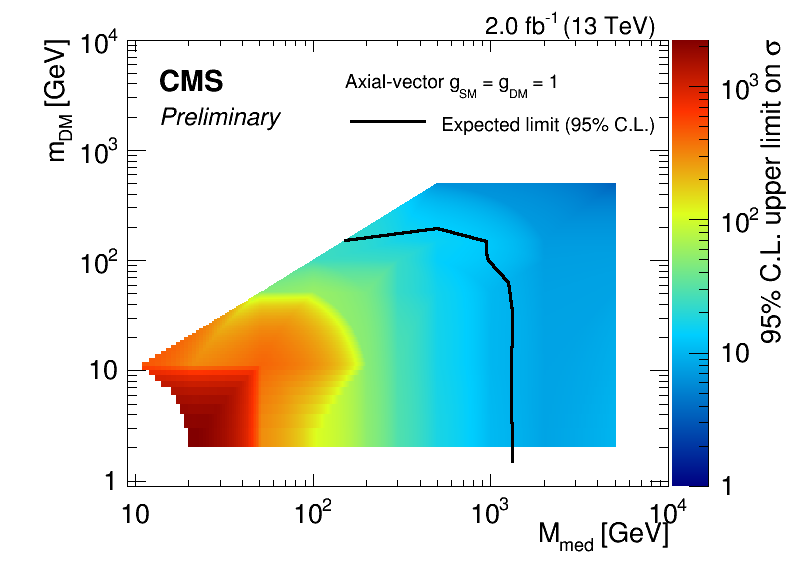
\includegraphics[width=0.75\textwidth]{figures/DMplots/dm_A_g1p0_2p0fb_2dlimits.png} \\
\caption{Expected 95\% CL upper limit on the cross section, and exclusion
contour for the axial-vector light flavour model with unity couplings at 2~\ifb.}
\label{fig:dm_A_g1_2fb_2dlimits}
\end{center}
\end{figure}

\begin{figure}
\begin{center}
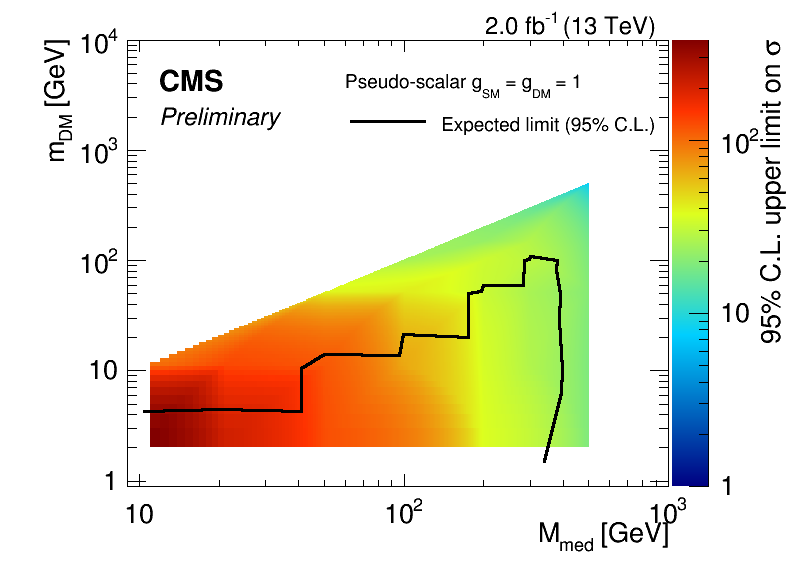
\includegraphics[width=0.75\textwidth]{figures/DMplots/dm_P_g1p0_2p0fb_2dlimits.png} \\
\caption{Expected 95\% CL upper limit on the cross section, and exclusion
contour for the pseudoscalar light flavour model with unity couplings at 2~\ifb.}
\label{fig:dm_P_g1_2fb_2dlimits}
\end{center}
\end{figure}




\clearpage
 \subsection{Heavy flavour models} \label{sec:dm_heavyjet}

Owing to the principal of Minimal Flavor Violation (MFV), top and bottom quarks
can play important roles in the phenomenology of dark matter. Scalar and
pseudoscalar models predict not only the `monojet' processes described in
Sec.~\ref{sec:dm_lightjet} but also the production of dark matter in association
with top (or bottom) pairs. This results in signatures with relatively large jet
multiplicities, in particular for \DMtt production. The \alphat analysis is well 
suited to searching for such signatures. An example Feynman diagram for the pair
production of dark matter particles in association with pairs of heavy quarks is
shown in Fig.~\ref{fig:feynman_hf}.


\begin{figure}[h!] \centering
\subfigure{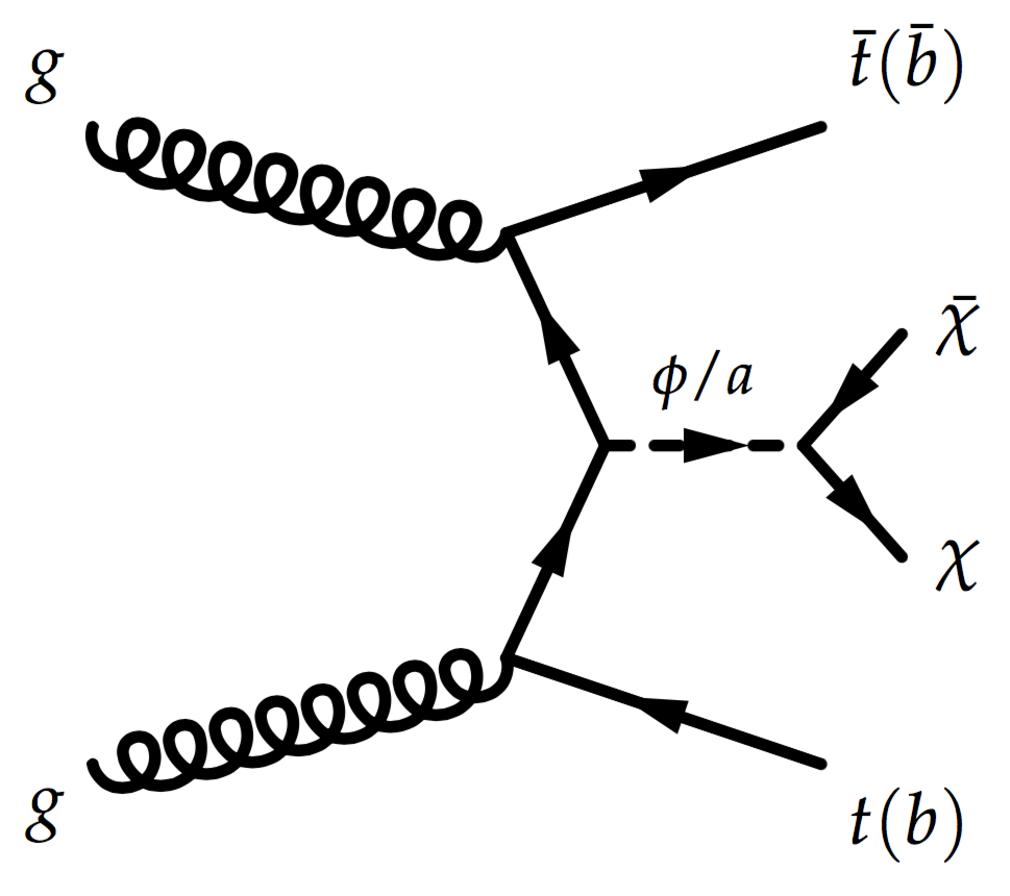
\includegraphics[width=0.35\textwidth]{figures/DMplots/feynman_hf.pdf}}
\caption{Feynman diagram of the pair production of Dark Matter particles in
association with $t\bar{t}$ or $b\bar{b}$. \cite{Abercrombie:2015wmb}}
\label{fig:feynman_hf} \end{figure}


The cross sections, signal yields and efficiencies for scalar and pseudoscalar
\DMtt models expected with 2~\ifb of data are shown in 
Tables~\ref{summaryTableAN_DMttP_xs10_2p1fb_exp}~and~\ref{summaryTableAN_DMttS_xs10_2p1fb_exp} for \DMtt. 

The selection efficiencies for these models are around $\sim 10$\%, and the improvement
provided by the new asymmetric and monojet categories is again evident.

\clearpage 
\begin{table}
\small
\centering
\begin{tabular}{lllllll}
\hline
$m_\phi$ & $m_\chi$ & $\sigma$ [pb] & Yield (sym) & Yield (asy) & Yield (mon) & Efficiency [\%] \\ \hline
100       &   10        &   1.90e-01  &   8.69      &   5.98      &   13.85     &   7.14      \\ 
10        &   10        &   1.50e-02  &   0.58      &   0.42      &   0.94      &   6.17      \\ 
50        &   10        &   3.03e-01  &   10.08     &   8.67      &   17.03     &   5.62      \\ 
200       &   150       &   4.12e-04  &   0.04      &   0.02      &   0.05      &   12.42     \\ 
500       &   150       &   4.61e-03  &   0.41      &   0.23      &   0.62      &   13.06     \\ 
100       &   1         &   1.91e-01  &   9.21      &   6.13      &   12.96     &   7.06      \\ 
10        &   1         &   4.41e-01  &   11.15     &   8.61      &   19.66     &   4.26      \\ 
200       &   1         &   8.36e-02  &   4.99      &   3.43      &   7.88      &   9.29      \\ 
20        &   1         &   3.99e-01  &   10.79     &   8.72      &   18.16     &   4.49      \\ 
300       &   1         &   4.00e-02  &   3.18      &   1.67      &   4.39      &   11.01     \\ 
500       &   1         &   5.41e-03  &   0.50      &   0.25      &   0.69      &   12.67     \\ 
50        &   1         &   3.03e-01  &   10.45     &   8.98      &   18.65     &   5.98      \\ 
500       &   500       &   3.27e-06  &   0.00      &   0.00      &   0.00      &   16.53     \\ 
200       &   50        &   8.38e-02  &   5.24      &   3.32      &   8.00      &   9.41      \\ 
300       &   50        &   3.99e-02  &   2.90      &   1.63      &   4.36      &   10.61     \\ 
50        &   50        &   2.98e-03  &   0.18      &   0.11      &   0.28      &   8.97      \\ 
\hline
\end{tabular}
\caption{Cross section, yields at 2~\ifb (split according to symmetric, asymmetric, and monojet categories), and total selection efficiency for the pseudo-scalar \DMtt samples.}
\label{summaryTableAN_DMttP_xs10_2p1fb_exp}
\end{table}

\begin{table}
\small
\centering
\begin{tabular}{lllllll}
\hline
$m_\phi$ & $m_\chi$ & $\sigma$ [pb] & Yield (sym) & Yield (asy) & Yield (mon) & Efficiency [\%] \\ \hline
100       &   10        &   6.73e-01  &   9.33      &   8.93      &   18.77     &   2.62      \\ 
10        &   10        &   9.49e-02  &   0.60      &   0.58      &   1.28      &   1.24      \\ 
50        &   10        &   2.94e+00  &   19.00     &   18.68     &   38.57     &   1.23      \\ 
200       &   150       &   1.30e-04  &   0.01      &   0.01      &   0.02      &   13.15     \\ 
500       &   150       &   3.75e-03  &   0.38      &   0.16      &   0.51      &   13.35     \\ 
1000      &   1         &   3.69e-04  &   0.05      &   0.02      &   0.06      &   15.60     \\ 
100       &   1         &   6.72e-01  &   11.19     &   8.06      &   19.68     &   2.76      \\ 
10        &   1         &   1.96e+01  &   39.91     &   49.57     &   71.29     &   0.39      \\ 
200       &   1         &   9.33e-02  &   4.63      &   2.47      &   7.05      &   7.22      \\ 
20        &   1         &   1.05e+01  &   23.20     &   37.53     &   63.82     &   0.57      \\ 
300       &   1         &   2.95e-02  &   2.28      &   1.10      &   3.13      &   10.52     \\ 
500       &   1         &   5.18e-03  &   0.49      &   0.23      &   0.70      &   13.02     \\ 
50        &   1         &   2.94e+00  &   20.38     &   20.31     &   34.00     &   1.21      \\ 
500       &   500       &   9.89e-07  &   0.00      &   0.00      &   0.00      &   16.94     \\ 
200       &   50        &   9.22e-02  &   5.17      &   2.72      &   7.55      &   7.97      \\ 
300       &   50        &   2.90e-02  &   2.31      &   1.12      &   3.36      &   11.16     \\ 
50        &   50        &   2.33e-03  &   0.10      &   0.06      &   0.14      &   6.13      \\ 
\hline
\end{tabular}
\caption{Cross section, yields at 2~\ifb (split according to symmetric, asymmetric, and monojet categories), and total selection efficiency for the scalar \DMtt samples.}
\label{summaryTableAN_DMttS_xs10_2p1fb_exp}
\end{table}
 
\clearpage


The yields and efficiencies for \DMbb are shown in Tables~\ref{summaryTableAN_DMbbP_xs10_2p1fb_exp}~and~\ref{summaryTableAN_DMbbS_xs10_2p1fb_exp}, respectively. 
\begin{table}
\small
\centering
\begin{tabular}{lllllll}
\label{summaryTableAN_DMbbP_xs10_2p1fb_exp}
\hline
$m_\phi$ & $m_\chi$ & $\sigma$ [pb] & Yield (sym) & Yield (asy) & Yield (mon) & Efficiency [\%] \\ \hline
1000      &   1000      &   2.31e-09  &   0.00      &   0.00      &   0.00      &   12.97     \\ 
10        &   1000      &   1.52e-09  &   0.00      &   0.00      &   0.00      &   13.18     \\ 
100       &   10        &   5.36e-01  &   0.08      &   0.17      &   0.61      &   0.08      \\ 
10        &   10        &   9.36e-02  &   0.00      &   0.01      &   0.02      &   0.01      \\ 
15        &   10        &   1.30e-01  &   0.00      &   0.01      &   0.02      &   0.01      \\ 
50        &   10        &   1.94e+00  &   0.04      &   0.11      &   0.50      &   0.02      \\ 
200       &   150       &   1.52e-04  &   0.00      &   0.00      &   0.00      &   1.46      \\ 
295       &   150       &   1.67e-03  &   0.01      &   0.01      &   0.02      &   1.03      \\ 
500       &   150       &   1.26e-03  &   0.01      &   0.01      &   0.04      &   2.11      \\ 
1000      &   1         &   5.48e-05  &   0.00      &   0.00      &   0.00      &   4.22      \\ 
100       &   1         &   5.37e-01  &   0.04      &   0.21      &   0.79      &   0.09      \\ 
10        &   1         &   6.25e+00  &   0.02      &   0.01      &   0.22      &   0.00      \\ 
200       &   1         &   8.59e-02  &   0.10      &   0.15      &   0.40      &   0.36      \\ 
20        &   1         &   4.82e+00  &   0.00      &   0.00      &   0.27      &   0.00      \\ 
300       &   1         &   2.25e-02  &   0.04      &   0.08      &   0.27      &   0.82      \\ 
500       &   1         &   1.51e-03  &   0.01      &   0.01      &   0.04      &   1.89      \\ 
50        &   1         &   1.95e+00  &   0.07      &   0.17      &   0.31      &   0.01      \\ 
10        &   500       &   2.12e-07  &   0.00      &   0.00      &   0.00      &   7.26      \\ 
500       &   500       &   3.10e-07  &   0.00      &   0.00      &   0.00      &   7.30      \\ 
995       &   500       &   6.70e-06  &   0.00      &   0.00      &   0.00      &   6.17      \\ 
10        &   50        &   3.19e-03  &   0.00      &   0.00      &   0.01      &   0.20      \\ 
200       &   50        &   8.56e-02  &   0.09      &   0.14      &   0.39      &   0.34      \\ 
50        &   50        &   4.19e-03  &   0.00      &   0.00      &   0.01      &   0.21      \\ 
95        &   50        &   2.21e-02  &   0.01      &   0.02      &   0.03      &   0.12      \\ 
\hline
\end{tabular}
\caption{Cross section, yields at 2~\ifb (split according to symmetric, asymmetric, and monojet categories), and total selection efficiency for the pseudo-scalar \DMbb samples.}
\label{summaryTableAN_DMbbP_xs10_2p1fb_exp}
\end{table}

\begin{table}
\small
\centering
\begin{tabular}{lllllll}
\hline
$m_\phi$ & $m_\chi$ & $\sigma$ [pb] & Yield (sym) & Yield (asy) & Yield (mon) & Efficiency [\%] \\ \hline
1000      &   1000      &   4.09e-10  &   0.00      &   0.00      &   0.00      &   13.48     \\ 
10        &   1000      &   2.88e-10  &   0.00      &   0.00      &   0.00      &   13.87     \\ 
100       &   10        &   1.24e+00  &   0.29      &   0.32      &   1.41      &   0.08      \\ 
10        &   10        &   2.68e-01  &   0.01      &   0.03      &   0.07      &   0.02      \\ 
15        &   10        &   3.52e-01  &   0.02      &   0.04      &   0.10      &   0.02      \\ 
50        &   10        &   7.66e+00  &   0.29      &   0.81      &   2.34      &   0.02      \\ 
200       &   150       &   5.91e-05  &   0.00      &   0.00      &   0.00      &   1.78      \\ 
295       &   150       &   2.58e-04  &   0.00      &   0.00      &   0.00      &   1.43      \\ 
500       &   150       &   1.50e-03  &   0.01      &   0.01      &   0.04      &   2.04      \\ 
1000      &   1         &   5.41e-05  &   0.00      &   0.00      &   0.00      &   4.44      \\ 
100       &   1         &   1.25e+00  &   0.37      &   0.49      &   1.75      &   0.10      \\ 
200       &   1         &   1.31e-01  &   0.08      &   0.23      &   0.63      &   0.34      \\ 
20        &   1         &   4.07e+01  &   0.00      &   1.41      &   0.56      &   0.00      \\ 
300       &   1         &   2.93e-02  &   0.06      &   0.11      &   0.32      &   0.79      \\ 
500       &   1         &   2.21e-03  &   0.01      &   0.02      &   0.06      &   2.00      \\ 
50        &   1         &   7.66e+00  &   0.87      &   0.44      &   1.10      &   0.02      \\ 
10        &   500       &   5.36e-08  &   0.00      &   0.00      &   0.00      &   8.61      \\ 
500       &   500       &   7.40e-08  &   0.00      &   0.00      &   0.00      &   8.27      \\ 
995       &   500       &   6.51e-07  &   0.00      &   0.00      &   0.00      &   6.72      \\ 
10        &   50        &   2.71e-03  &   0.00      &   0.00      &   0.01      &   0.32      \\ 
50        &   50        &   3.37e-03  &   0.00      &   0.01      &   0.01      &   0.29      \\ 
95        &   50        &   1.04e-02  &   0.01      &   0.01      &   0.03      &   0.19      \\ 
\hline
\end{tabular}
\caption{Cross section, yields at 2~\ifb (split according to symmetric, asymmetric, and monojet categories), and total selection efficiency for the pseudo-scalar \DMtt samples.}
\label{tab:dm_DMttP_g1_2fb}
\end{table}
 
\clearpage


\subsubsection{Expected and observed sensitivities for DM+$t\bar{t}$}

The expected 95\% CL signal strength limits for simplified \DMtt models with scalar and
pseudo-scalar couplings are calculated for 2~\ifb. An uncertainty of 20\% is assumed for all 
heavy quark samples.


%These are shown in Tables~\ref{tab:dm_DMttS_2fb_limits}~and~\ref{tab:dm_DMttP_2fb_limits}. At this
%integrated luminosity, the sensitivity approaches scalar mediator masses of up 
%to 100~GeV and DM masses of about 10 GeV, whereas it is insufficient to
%significantly exclude the pseudoscalar model, which has generally smaller cross
%sections.

%Figure~\ref{fig:dm_DMttS_2fb_2dlimits} shows the interpolated scalar expected exclusion contour in the {\mphi-\mchi} mass plane.


\clearpage
Expected limits obtained for DM+$t\bar{t}$ are given in Tables~\ref{limits_DMttP_xs10_2p1fb_exp}-\ref{limits_DMttS_xs10_2p1fb_exp}, corresponding observed limits are shown in Tables~\ref{limits_DMttP_xs10_2p1fb_obs}-\ref{limits_DMttS_xs10_2p1fb_obs}.
\begin{table}
\begin{center}
\caption{DMttP xs10 2p1fb exp 95\% CL upper limits}
\begin{tabular}{lcccccccc}
\label{limits_DMttP_xs10_2p1fb_exp}
\multirow{5}{*}{\rotatebox{90}{$m_{\rm{DM}}$ (GeV)}}
& \multicolumn{1}{c|}{500} &  &  &  &  &  &  & 2.83e+04\\ 
& \multicolumn{1}{c|}{150} &  &  &  &  & 509.12 &  & 37.06\\ 
& \multicolumn{1}{c|}{50} &  &  & 116.37 &  & 3.90 & 7.22 & \\ 
& \multicolumn{1}{c|}{10} & 42.02 &  & 2.27 & 2.80 &  &  & \\ 
& \multicolumn{1}{c|}{1} & 1.83 & 2.21 & 2.37 & 2.69 & 4.15 & 5.98 & 35.21\\ 
\cline{2-9}
& \multicolumn{1}{c|}{} & 10 & 20 & 50 & 100 & 200 & 300 & 500\\ 
& & \multicolumn{6}{c}{$M_{\rm{Med}}$ (GeV)}
\end{tabular}
\end{center}
\end{table}


\begin{table}
\begin{center}
\caption{DMttS 2.1\ifb exp 95\% CL upper limits}
\begin{tabular}{lccccccccc}
\label{limits_DMttS_xs10_2p1fb_exp}
\multirow{5}{*}{\rotatebox{90}{$m_{\rm{DM}}$ (GeV)}}
& \multicolumn{1}{c|}{500} &  &  &  &  &  &  & 9.38e+04 & \\ 
& \multicolumn{1}{c|}{150} &  &  &  &  & 1.24e+03 &  & 42.92 & \\ 
& \multicolumn{1}{c|}{50} &  &  & 207.56 &  & 4.29 & 8.25 &  & \\ 
& \multicolumn{1}{c|}{10} & 24.40 &  & 0.89 & 1.97 &  &  &  & \\ 
& \multicolumn{1}{c|}{1} & 0.38 & 0.49 & 0.77 & 2.06 & 4.97 & 8.77 & 34.88 & 304.60\\ 
\cline{2-10}
& \multicolumn{1}{c|}{} & 10 & 20 & 50 & 100 & 200 & 300 & 500 & 1000\\ 
& & \multicolumn{7}{c}{$M_{\rm{Med}}$ (GeV)}
\end{tabular}
\end{center}
\end{table}


\begin{table}
\begin{center}
\caption{DMttP 2.1\ifb obs 95\% CL upper limits}
\begin{tabular}{lcccccccc}
\label{limits_DMttP_xs10_2p1fb_obs}
\multirow{5}{*}{\rotatebox{90}{$m_{\rm{DM}}$ (GeV)}}
& \multicolumn{1}{c|}{500} &  &  &  &  &  &  & 4.79e+04\\ 
& \multicolumn{1}{c|}{150} &  &  &  &  & 710.48 &  & 78.72\\ 
& \multicolumn{1}{c|}{50} &  &  & 149.04 &  & 8.18 & 10.45 & \\ 
& \multicolumn{1}{c|}{10} & 67.24 &  & 3.15 & 5.38 &  &  & \\ 
& \multicolumn{1}{c|}{1} & 3.03 & 4.43 & 3.38 & 4.65 & 5.96 & 10.28 & 58.06\\ 
\cline{2-9}
& \multicolumn{1}{c|}{} & 10 & 20 & 50 & 100 & 200 & 300 & 500\\ 
& & \multicolumn{6}{c}{$M_{\rm{Med}}$ (GeV)}
\end{tabular}
\end{center}
\end{table}


\begin{table}
\begin{center}
\caption{DMttS 2.1\ifb obs 95\% CL upper limits}
\begin{tabular}{lccccccccc}
\label{limits_DMttS_xs10_2p1fb_obs}
\multirow{5}{*}{\rotatebox{90}{$m_{\rm{DM}}$ (GeV)}}
& \multicolumn{1}{c|}{500} &  &  &  &  &  &  & 1.37e+05 & \\ 
& \multicolumn{1}{c|}{150} &  &  &  &  & 2.53e+03 &  & 75.92 & \\ 
& \multicolumn{1}{c|}{50} &  &  & 466.29 &  & 9.64 & 17.03 &  & \\ 
& \multicolumn{1}{c|}{10} & 40.07 &  & 1.33 & 4.20 &  &  &  & \\ 
& \multicolumn{1}{c|}{1} & 0.45 & 0.99 & 1.27 & 3.99 & 11.27 & 14.34 & 47.10 & 539.73\\ 
\cline{2-10}
& \multicolumn{1}{c|}{} & 10 & 20 & 50 & 100 & 200 & 300 & 500 & 1000\\ 
& & \multicolumn{7}{c}{$M_{\rm{Med}}$ (GeV)}
\end{tabular}
\end{center}
\end{table}




Appendix~\ref{sec:dm_checklist} contains additional validation of the \DMj DM samples like signal and background yields for the most sensitive bins and sensitivities.

\subsubsection{Expected and observed sensitivities for DM+$b(\bar{b})$}

The expected 95\% CL signal strength limits for simplified DM+$t(\bar{t})$ models with scalar and
pseudo-scalar couplings are calculated for 2~\ifb. An uncertainty of 20\% is assumed for all 
heavy quark samples.


Figure~\ref{fig:dm_DMttS_2fb_2dlimits} shows the interpolated scalar expected 
exclusion contour in the {\mphi-\mchi} mass plane.


\clearpage
Expected limits obtained for DM+$t\bar{t}$ are given in Tables~\ref{limits_DMbbP_xs10_2p1fb_exp}-\ref{limits_DMbbS_xs10_2p1fb_exp}, corresponding observed limits are shown in Tables~\ref{limits_DMbbP_xs10_2p1fb_obs}-\ref{limits_DMbbS_xs10_2p1fb_ob}.
\begin{table}
\begin{center}
\tiny
\caption{DMbbP xs10 2p1fb exp 95\% CL upper limits}
\begin{tabular}{lccccccccccccc}
\label{limits_DMbbP_xs10_2p1fb_exp}
\multirow{6}{*}{\rotatebox{90}{$m_{\rm{DM}}$ (GeV)}}
& \multicolumn{1}{c|}{1000} & 2.03e+08 &  &  &  &  &  &  &  &  &  &  & 1.44e+08\\ 
& \multicolumn{1}{c|}{500} & 3.76e+06 &  &  &  &  &  &  &  &  & 2.79e+06 & 1.67e+05 & \\ 
& \multicolumn{1}{c|}{150} &  &  &  &  &  &  & 3.14e+04 & 5.07e+03 &  & 3.16e+03 &  & \\ 
& \multicolumn{1}{c|}{50} & 6.87e+03 &  &  & 5.53e+03 & 1.50e+03 &  & 162.84 &  &  &  &  & \\ 
& \multicolumn{1}{c|}{10} & 1.60e+03 & 827.41 &  & 156.65 &  & 105.24 &  &  &  &  &  & \\ 
& \multicolumn{1}{c|}{1} & 177.94 &  & 78.47 & 70.34 &  & 93.38 & 180.58 &  & 415.85 & 2.64e+03 &  & 3.36e+04\\ 
\cline{2-14}
& \multicolumn{1}{c|}{} & 10 & 15 & 20 & 50 & 95 & 100 & 200 & 295 & 300 & 500 & 995 & 1000\\ 
& & \multicolumn{11}{c}{$M_{\rm{Med}}$ (GeV)}
\end{tabular}
\end{center}
\end{table}

\begin{table}
\begin{center}
\tiny
\caption{DMbbS xs10 2p1fb exp 95\% CL upper limits}
\begin{tabular}{lccccccccccccc}
\label{limits_DMbbS_xs10_2p1fb_exp}
\multirow{6}{*}{\rotatebox{90}{$m_{\rm{DM}}$ (GeV)}}
& \multicolumn{1}{c|}{1000} & 1.03e+09 &  &  &  &  &  &  &  &  &  &  & 7.52e+08\\ 
& \multicolumn{1}{c|}{500} & 1.27e+07 &  &  &  &  &  &  &  &  & 1.08e+07 & 1.48e+06 & \\ 
& \multicolumn{1}{c|}{150} &  &  &  &  &  &  & 6.97e+04 & 2.12e+04 &  & 2.72e+03 &  & \\ 
& \multicolumn{1}{c|}{50} & 7.24e+03 &  &  & 5.96e+03 & 2.09e+03 &  &  &  &  &  &  & \\ 
& \multicolumn{1}{c|}{10} & 828.51 & 210.29 &  & 24.07 &  & 43.11 &  &  &  &  &  & \\ 
& \multicolumn{1}{c|}{1} & -1.00 &  & 21.19 & 11.30 &  & 38.25 & 161.04 &  & 290.34 & 1.85e+03 &  & 3.10e+04\\ 
\cline{2-14}
& \multicolumn{1}{c|}{} & 10 & 15 & 20 & 50 & 95 & 100 & 200 & 295 & 300 & 500 & 995 & 1000\\ 
& & \multicolumn{11}{c}{$M_{\rm{Med}}$ (GeV)}
\end{tabular}
\end{center}
\end{table}


\begin{table}
\begin{center}
\tiny
\caption{DMbbP xs10 2p1fb obs 95\% CL upper limits}
\begin{tabular}{lccccccccccccc}
\label{limits_DMbbP_xs10_2p1fb_obs}
\multirow{6}{*}{\rotatebox{90}{$m_{\rm{DM}}$ (GeV)}}
& \multicolumn{1}{c|}{1000} & 3.41e+08 &  &  &  &  &  &  &  &  &  &  & 2.04e+08\\ 
& \multicolumn{1}{c|}{500} & 4.68e+06 &  &  &  &  &  &  &  &  & 3.95e+06 & 2.12e+05 & \\ 
& \multicolumn{1}{c|}{150} &  &  &  &  &  &  & 6.05e+04 & 6.78e+03 &  & 5.75e+03 &  & \\ 
& \multicolumn{1}{c|}{50} & 6.69e+03 &  &  & 5.39e+03 & 1.29e+03 &  & 232.75 &  &  &  &  & \\ 
& \multicolumn{1}{c|}{10} & 1.93e+03 & 966.61 &  & 239.84 &  & 111.76 &  &  &  &  &  & \\ 
& \multicolumn{1}{c|}{1} & 381.09 &  & 55.43 & 79.27 &  & 142.25 & 213.16 &  & 430.82 & 3.23e+03 &  & 6.82e+04\\ 
\cline{2-14}
& \multicolumn{1}{c|}{} & 10 & 15 & 20 & 50 & 95 & 100 & 200 & 295 & 300 & 500 & 995 & 1000\\ 
& & \multicolumn{11}{c}{$M_{\rm{Med}}$ (GeV)}
\end{tabular}
\end{center}
\end{table}

\begin{table}
\begin{center}
\tiny
\caption{DMbbS 2.1\ifb obs 95\% CL upper limits}
\begin{tabular}{lccccccccccccc}
\label{limits_DMbbS_xs10_2p1fb_obs}
\multirow{6}{*}{\rotatebox{90}{$m_{\rm{DM}}$ (GeV)}}
& \multicolumn{1}{c|}{1000} & 1.63e+09 &  &  &  &  &  &  &  &  &  &  & 1.02e+09\\ 
& \multicolumn{1}{c|}{500} & 2.43e+07 &  &  &  &  &  &  &  &  & 1.12e+07 & 2.93e+06 & \\ 
& \multicolumn{1}{c|}{150} &  &  &  &  &  &  & 7.75e+04 & 3.59e+04 &  & 5.32e+03 &  & \\ 
& \multicolumn{1}{c|}{50} & 1.50e+04 &  &  & 8.42e+03 & 3.25e+03 &  &  &  &  &  &  & \\ 
& \multicolumn{1}{c|}{10} & 1.66e+03 & 283.08 &  & 15.68 &  & 32.64 &  &  &  &  &  & \\ 
& \multicolumn{1}{c|}{1} & 274.77 &  & 30.34 & 21.62 &  & 75.28 & 385.14 &  & 407.13 & 3.84e+03 &  & 5.11e+04\\ 
\cline{2-14}
& \multicolumn{1}{c|}{} & 10 & 15 & 20 & 50 & 95 & 100 & 200 & 295 & 300 & 500 & 995 & 1000\\ 
& & \multicolumn{11}{c}{$M_{\rm{Med}}$ (GeV)}
\end{tabular}
\end{center}
\end{table}



Appendix~\ref{sec:dm_checklist} contains additional validation for the \DMtt and \DMtt DM samples like signal and background yields for the most sensitive bins and sensitivities.

